%\documentclass[10pt, handout]{beamer}
\documentclass[10pt]{beamer}
% use the first one to ignore /pause and the second one to make use of it!
\usetheme[
%%% option passed to the outer theme
%    progressstyle=fixedCircCnt,   % fixedCircCnt, movingCircCnt (moving is deault)
  ]{Feather}
  
% If you want to change the colors of the various elements in the theme, edit and uncomment the following lines

% Change the bar colors:
%\setbeamercolor{Feather}{fg=red!100,bg=red!0}

% Change the color of the structural elements:
\setbeamercolor{structure}{fg=white}

% Change the frame title text color:
\setbeamercolor{frametitle}{fg=white}

% Change the normal text color background:
\setbeamercolor{normal text}{fg=white, bg= }%gray!90}

\definecolor{light-gray}{gray}{0.7}

%-------------------------------------------------------
% INCLUDE PACKAGES
%-------------------------------------------------------

\usepackage[utf8]{inputenc}
\usepackage[ngerman]{babel}
\usepackage[T1]{fontenc}
\usepackage{helvet}
\usepackage{array}

\usepackage{media9} %for video playback (only working with acrobat

\usepackage{pdfpages}

\usepackage{listings}
%\usepackage{fancyhdr}
%\usepackage{tikz}
%\usepackage{tkz-graph}
%\usetikzlibrary{calc}
%\usetikzlibarary{calc}

%-------------------------------------------------------
% DEFFINING AND REDEFINING COMMANDS
%-------------------------------------------------------

% colored hyperlinks
\newcommand{\chref}[2]{
  \href{#1}{{\usebeamercolor[bg]{Feather}#2}}
}



%-------------------------------------------------------
% INFORMATION IN THE TITLE PAGE
%-------------------------------------------------------

\title[Lego Car] % [] is optional - is placed on the bottom of the sidebar on every slide
{ % is placed on the title page
      \textbf{Lego Car}
}

\subtitle[Final Presentation]
{
      \textbf{Final Presentation}
}

\author[Autor]
{      
	Moritz Dötterl, Berkay Sümer, Abdallah Emad, Heiko Lengenfelder
}

%\institute[]
%{
%       "Estar no estado de graça concede ao homem o céu no futuro; saber que está no estado de graça concede o céu agora e no futuro". - Thomas Brooks (Livro "Céu na Terra" de 1654)
  
  %there must be an empty line above this line - otherwise some unwanted space is added between the university and the country (I do not know why;( )
%}

\date{27.6.2016}


%-------------------------------------------------------
% THE BODY OF THE PRESENTATION
%-------------------------------------------------------



\begin{document}

%-------------------------------------------------------
% THE TITLEPAGE
%-------------------------------------------------------

{\1% % this is the name of the PDF file for the background
\begin{frame}[plain,noframenumbering] % the plain option removes the header from the title page, noframenumbering removes the numbering of this frame only
  \titlepage % call the title page information from above
\end{frame}

{
\addtobeamertemplate{navigation symbols}{}{%
%\addtobeamertemplate{footline}{%
    \usebeamerfont{footline}%
    \usebeamercolor[fg]{title}%
   \small\insertframenumber%/\inserttotalframenumber
   \hspace{6,28cm}%
}

\begin{frame}[plain]{\huge Agenda}
	\begin{itemize}
	\LARGE
		\item Hardware \& Wiring
		\item Adaptive Cruse Control
		\item Steering Control
		\item Optimizations
	\end{itemize}

\end{frame}

%\iffalse
% 
\begin{frame}[plain]{Wiring}{overview}
	Components:
	\center
	\pause
	\begin{itemize}
		\item Sensors
		\begin{itemize}
			\item Ultrasonic
			\item Camera
		\end{itemize}
		\pause
		\item Actuators
		\begin{itemize}
			\item Steering Servo
			\item Drive Motor
		\end{itemize}
		\pause
		\item Controll
		\begin{itemize}
			\item Nanoboard
			\item Raspberry Pi
		\end{itemize}
		\pause
		\item Power supply
		\begin{itemize}
			\item Battery
			\item H-Bridge
		\end{itemize}
	\end{itemize}
	
\end{frame}
 
 
 \begin{frame}[plain]{Wiring}{circuit layout}
	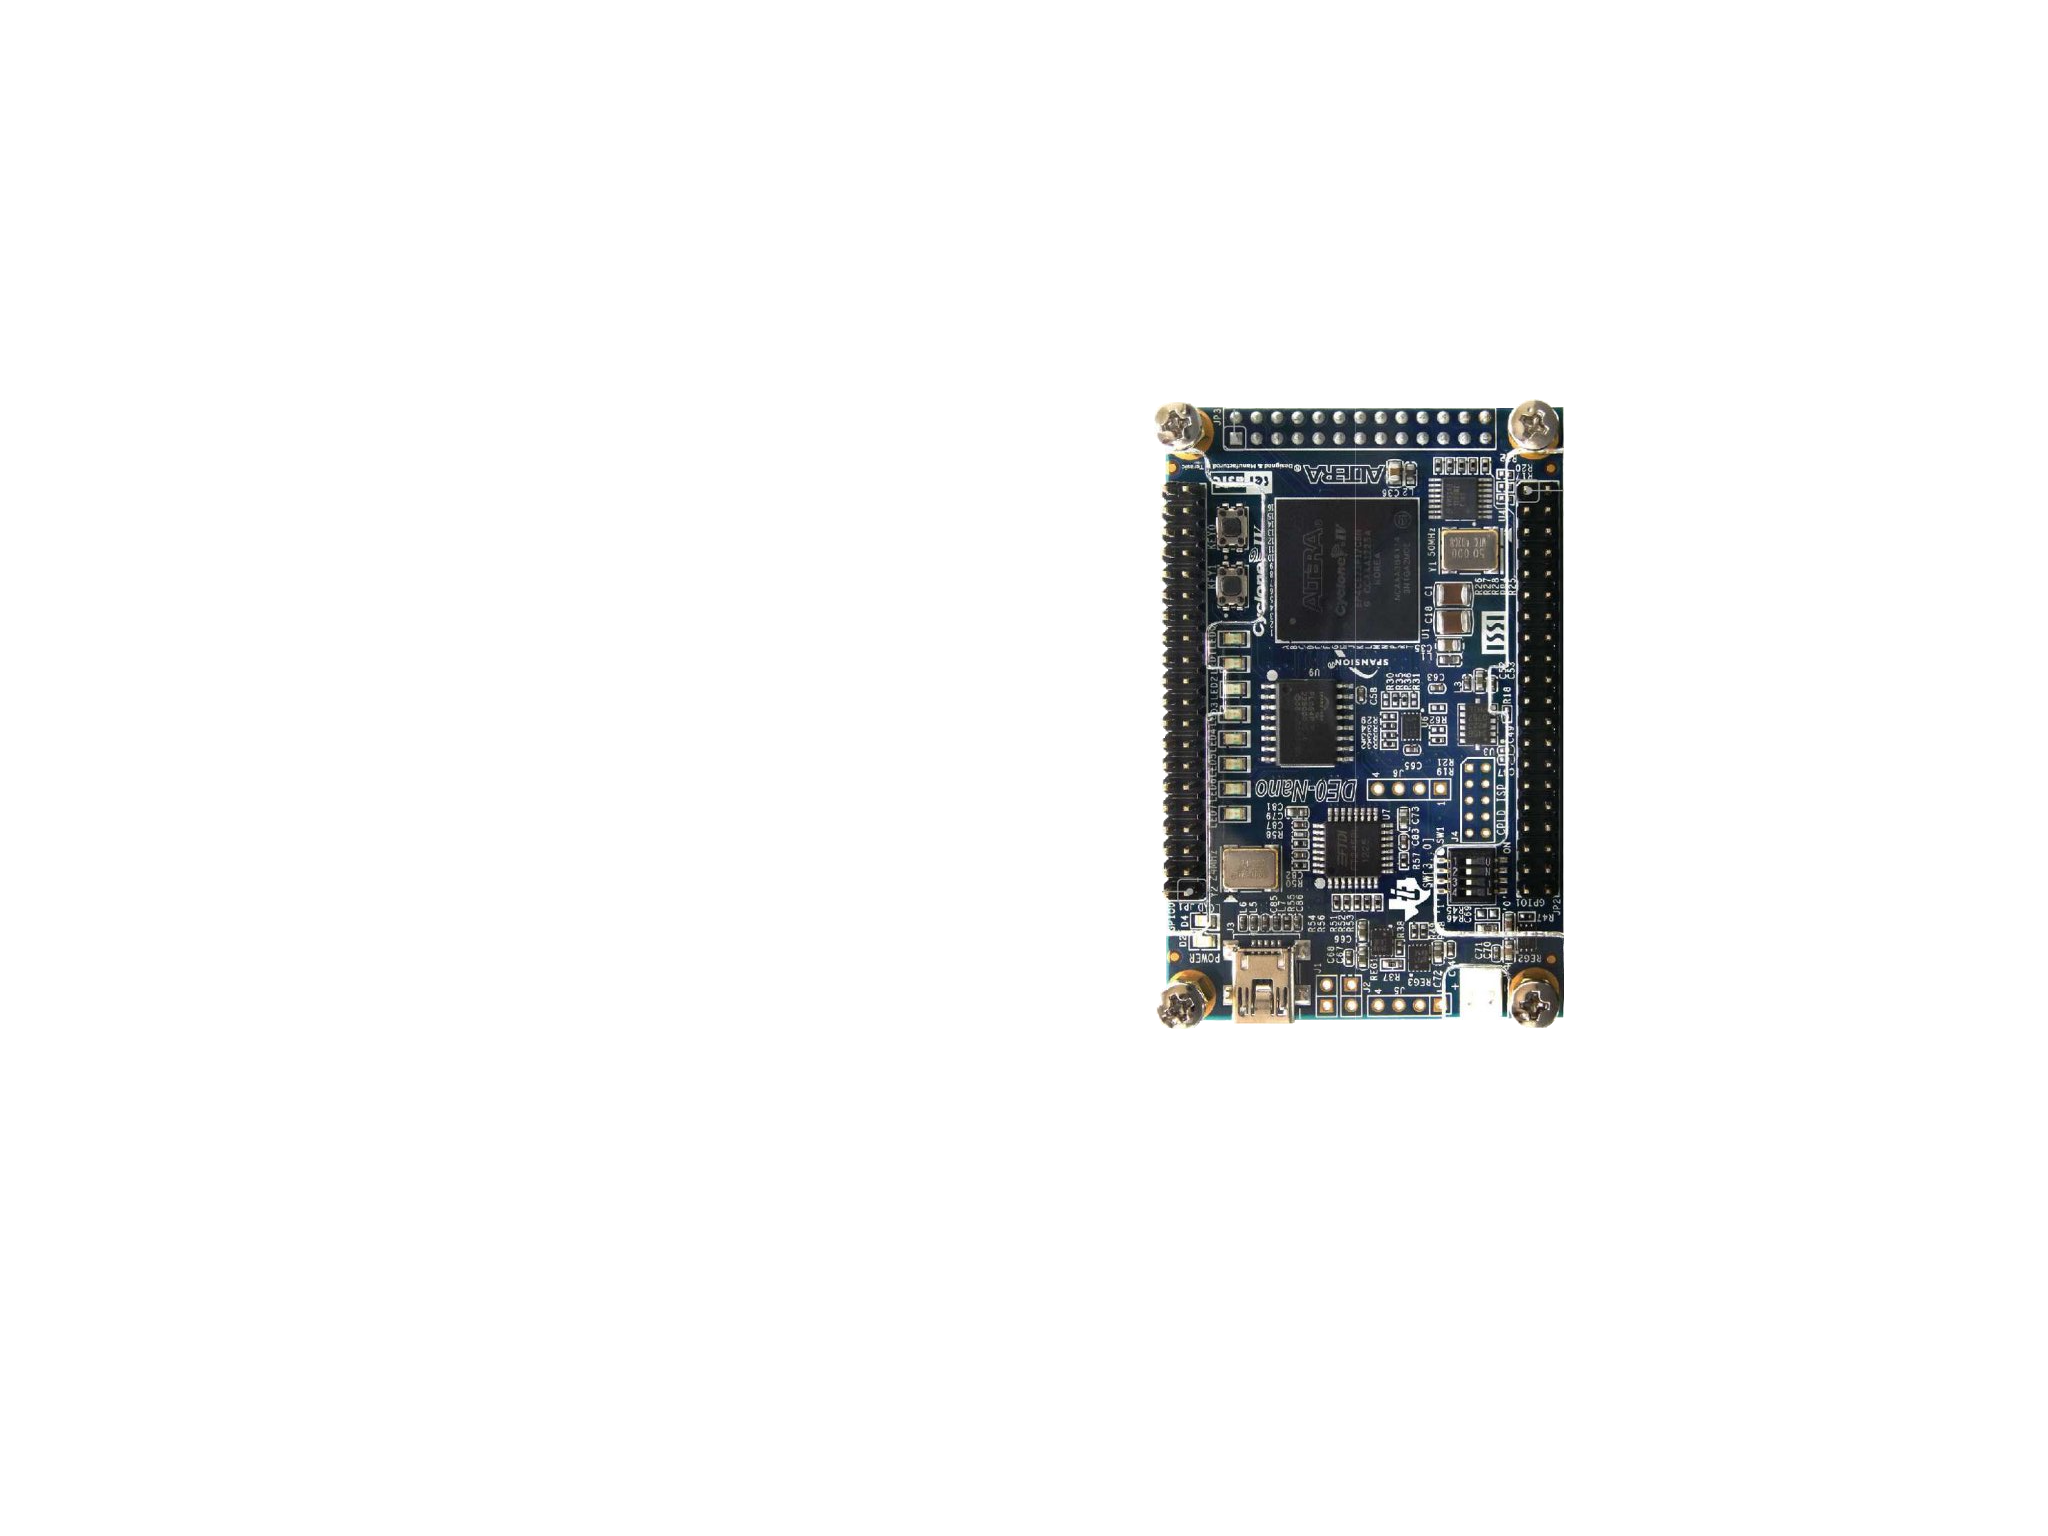
\includegraphics[width=\textwidth]{Feathergraphics/wiring1}
	\end{frame}
	
	
 \newcounter{ctra}
\setcounter{ctra}{2}
\whiledo {\value{ctra} < 13}%
{%
\begin{frame}[plain,noframenumbering]{Wiring}{circuit layout}
	\includegraphics[width=\textwidth]{Feathergraphics/wiring\the\value{ctra}}

\end{frame}
 \stepcounter {ctra}%
}
\addtocounter{page}{-16}

}}
{
\addtobeamertemplate{navigation symbols}{}{%
    \usebeamerfont{footline}%
    \usebeamercolor[fg]{title}%
   \small\insertframenumber%/\inserttotalframenumber
   \hspace{6,28cm}%
}

\includepdf[pages=-,pagecommand={\setcounter{framenumber}{\value{page}}\thispagestyle{plain}}]{berkay_endterm.pdf}


{\1
%\fi
 
\begin{frame}[plain]{Raspberry Pi}
	% this is a comment
	\begin{itemize}
		\item Raspberry Pi Version: Raspberry Pi 3
		\item Capable little computer that can be used for electronics projects
		\item Used to connect the camera with the nano-board for the line detection
	\end{itemize}
	
	\begin{figure}
	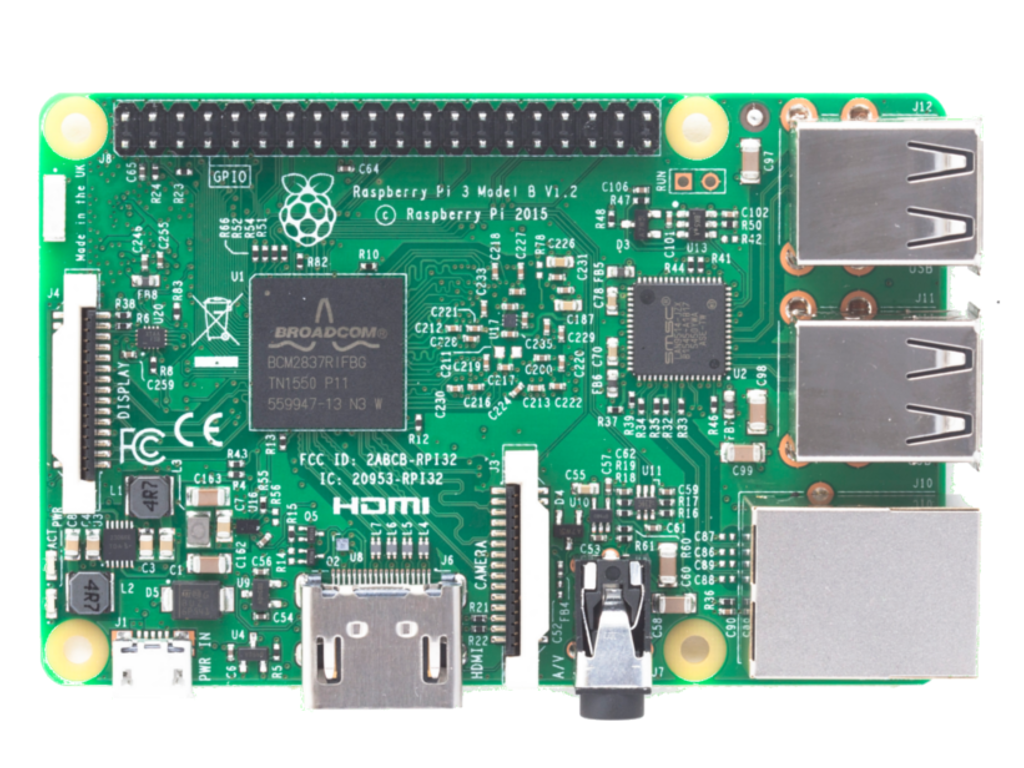
\includegraphics[width=7cm, height=5cm]{raspi2.png}
	\end{figure}
	
	\vspace{2cm}
	this text has 2cm Distance from above (because of vspace)\\ % \\ means new line
	Abdallah
\end{frame}

\begin{frame}[plain]{Raspberry Pi}

Carried out steps:
\begin{enumerate}
		\item Raspbian installed (operating system for the Raspberry Pi)
		\item Connected to the laptop using Ethernet
		\item Used SSH (Secure Shell) to gain access to the command line of the Raspberry Pi
		\item Controlled the Raspberry Pi using VNC (a graphical desktop sharing system)
		\item Downloaded OpenCV and connected the camera
		\item Tested the Code for the line detection
	\end{enumerate}
	

	
To-Do:
\begin{enumerate}
		\item Connect the Raspberry Pi to the nano-board
		\item Align the line detection with the motor control
	\end{enumerate}

\end{frame}

\begin{frame}[plain]{Raspberry Pi}
\begin{figure}
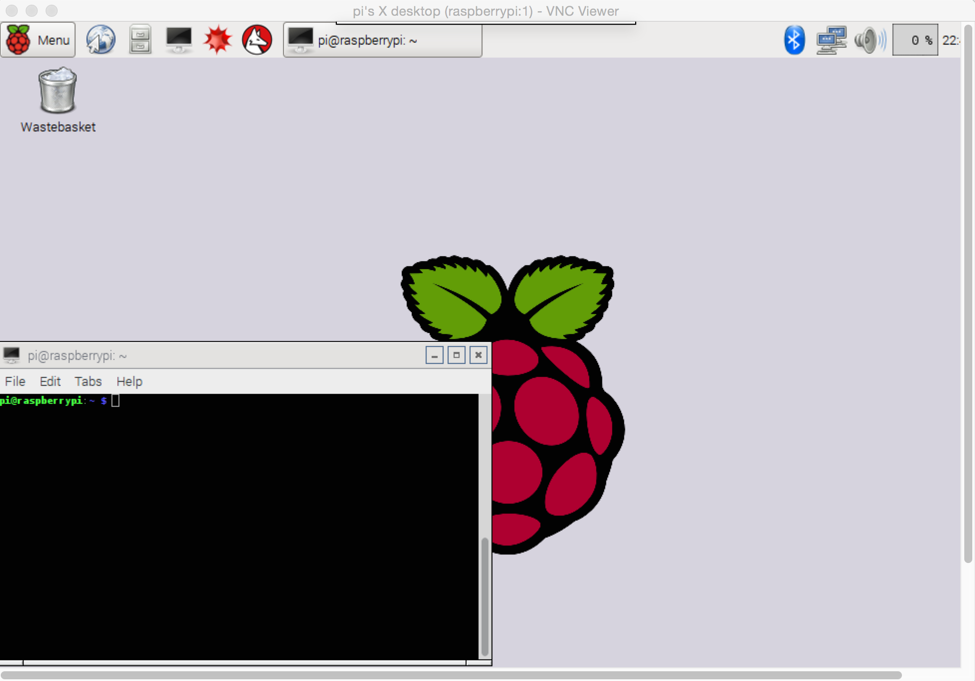
\includegraphics[width=8cm, height=7cm]{vnc.png}
\end{figure}	
\end{frame}

\begin{frame}[plain]{Steering Control}
	% this is a comment
	\large 
	\textbf{Approach}
	\begin{itemize}
		\item Approximate line
		\item Calculate direction
		\item Send data to Nano-Board
	\end{itemize}
	\pause
	\textbf{Assumptions}
	\begin{itemize}
		\item Vertical line
		\item Car position
		\item Line is highest contrast on image
	\end{itemize}
	\pause
	\textbf{Tools}
	\begin{itemize}
		\item Code in C++
		\item OpenCV
	\end{itemize}
\end{frame}

\begin{frame}[plain]{Steering Control}
	\large 
	\textbf{Algorithm}	
	\begin{enumerate}
		\item Get frame of camera (15 fps)
		\pause
		\item Blur Image
				\begin{itemize}
					\item Could be done by Gaussian-Filter
					\item Do it by hardware (faster)
				\end{itemize}
		\pause
		\item Convert Image from RGB to gray
		\pause
		\item Approximate gradient
				\begin{itemize}
					\item Only horizontal change
					\item Apply Mask
							$
							M=
							\begin{bmatrix}
							-1 & 0 & 1 \\
							-2 & 0 & 2 \\
							-1 & 0 & 1
							\end{bmatrix}
							$
				\end{itemize}
		\pause
		\item Find maximum value each row
				\begin{itemize}
					\item Store points
					\item Threshold for max x,y-distance
					\item Threshold for min gradient value
				\end{itemize}
	\end{enumerate}
\end{frame}	

\begin{frame}[plain]{Steering Control}
	\large
	\textbf{Algorithm}
	\begin{enumerate}
		\setcounter{enumi}{5}
		\item Fit line on points (squared distance weighting)
		\pause
		\item Calculate steering angle
		\pause
		\item Add angle: $SteeringAngle = \alpha * NewAngle + (1-\alpha) * LastAngle$
		\pause
		\item Map angle to servo levels (15 settings)
		\pause
		\item Send via Uart
	\end{enumerate}
	\pause
	\textbf{Parameters}
	\begin{itemize}
		\item Weight of new angle ($\alpha$)
		\item Threshold for distance and gradients
		\item Mapping (linear, progressing)
		\item Number of threads
	\end{itemize}
\end{frame}

%\begin{frame}[plain]{Line Detection}
%	\begin{columns}[T]
%		\begin{column}[T]{5cm}
%			\vspace{5mm}
%			Steps
%			\begin{itemize}				
%				\visible<1->{\item Get Frame from camera}
%				\visible<2->{\item Apply Gaussian Filter}
%				\visible<3->{\item Transform image from RGB to grey}
%				\visible<4->{
%				\item Approximate Gradient
%					$
%					M=
%					\begin{bmatrix}
%					-1 & 0 & 1 \\
%					-2 & 0 & 2 \\
%					-1 & 0 & 1
%					\end{bmatrix}
%					$			
%				}
%				\visible<5->{\item Calculate maximal points for each row}
%				\visible<6->{\item Fit line on points}
%				\visible<7->{\item Calculate direction of car}
%			\end{itemize}
%		\end{column}
%		\begin{column}[T]{7cm}
%			\vspace{1cm}
%			\includegraphics<1>[width=\textwidth]{Heikographics/line1}
%			\includegraphics<2>[width=\textwidth]{Heikographics/line2}
%			\includegraphics<3>[width=\textwidth]{Heikographics/line3}
%			\includegraphics<4>[width=\textwidth]{Heikographics/line4}
%			\includegraphics<5>[width=\textwidth]{Heikographics/line5}
%			\includegraphics<6>[width=\textwidth]{Heikographics/line6}
%			\includegraphics<7>[width=\textwidth]{Heikographics/line7}
%		\end{column}
%	\end{columns}
%\end{frame}





\begin{frame}[plain]{Optimization Strategies}{Troubleshooting}
\large
\pause
	First tests: Not so good...\\
	\pause
	Why does the car lose the line?\\
	\pause
	Use laptop instead of Raspberry Pi: 
		\pause
		\begin{itemize}
			\large
			\item Car worked perfectly fine
			\pause
			\item Reason: 
			\pause
			\begin{itemize}
				\large
				\item Computation power
				\pause
				\item $\approx$ 4ms per frame \pause (Pi: $\approx$170ms)
				\pause
				\item Camera: 15 FPS \pause $\Rightarrow$ new frame every 66ms
			\end{itemize}	
			\pause
			\item BUT: Algorithm concept works!
			
		\end{itemize}		 
\end{frame}
 
  
\begin{frame}[plain]{Optimization Strategies}{Guideline}
\large
	Main Problems:
	\pause
	\begin{itemize}
	\large
		\item Runtime
		\begin{itemize}
		\large
			\item Reaction time $\Leftrightarrow$ feasible speed
		\end{itemize}
		\pause
		\item Not all frames of the camera are processed
	\end{itemize}
	\pause
	\vspace{1.5cm}
	Main Improvements:
	\pause
	\begin{itemize}
	\large
		\item Improve runtime
		\begin{itemize}
		\large
			\item Improve reaction time $\Leftrightarrow$ feasible speed
		\end{itemize}
		\pause
		\item Process every frame
		\begin{itemize}
		\large
			\item Improve feasible speed
		\end{itemize}
	\end{itemize}
	
\end{frame}

\begin{frame}[plain]{Optimization Strategies}{Optimize Runtime}
\large
\pause
Disabled Gaussian Filter
\pause
\begin{itemize}
	\large
	\item Saves a lot of computation time
	\pause
	\item Replaced it by simple hardware trick
	\pause
	\begin{itemize}
		\large
		\item changed focus of camera \pause $\Rightarrow$ image gets blurred
	\end{itemize}
\end{itemize}
\pause
Restrict search range 
\pause
\begin{itemize}
	\large
	\item Before: search total line for largest Gradient
	\pause
	\item Now: only search at x-Position of last line $\pm$80 pixels
\end{itemize}
\pause
Only consider Gradients >25
\pause
\begin{itemize}
	\large
	\item If not found in search range: ignore line
\end{itemize}
\end{frame}

\begin{frame}[plain]{Optimization Strategies}{exploit concurrency}
\large
\pause
	Optimized runtime: $\approx$100-110ms per frame
	\pause
	\begin{itemize}
		\large
		\item Pretty good, but still every second frame lost
		\pause
		\item We are only using one core\pause, but Raspberry Pi has 4!
	\end{itemize}
	\pause
	\vspace{.5cm}
	Recompile OpenCV WITH\_OPENMP
	\pause
	\begin{itemize}
		\large
		\item Uses OpenMP to parallelize OpenCV calls
		\pause
		\item Runtime: $\approx$80ms 
		\pause
		\item still >66ms \pause $\Rightarrow$ Not good enough
	\end{itemize}
	
\end{frame}

\begin{frame}[plain]{Optimization Strategies}{exploit concurrency}
\pause
%\large
If we can't catch all frames with one thread why not use two?
\vspace{.5cm}
\begin{itemize}
	\pause
	\item Main thread starts two worker threads and sleeps
	\pause
	\item Worker thread grabs a image from the camera (synchronized)
	\pause
	\item Worker processes the image 
	\pause
	\item Worker checks whether a later frame had already finished
	\pause
	\item Worker wakes Main thread and communicates the calculated direction
	\pause
	\item Main thread generates UART signal and sleeps again
\pause
\end{itemize}
\vspace{.5cm}
This does not affect Reaction time, but increases performance
\end{frame}

\begin{frame}[plain]{Optimization Strategies}{exploit concurrency}
\pause
	Our approach and the WITH\_OPENMP option don't work well together
	\pause
		\begin{itemize}
			\item Runtime $\approx$120-130ms per frame (using 2 threads)
			\pause
			\item Probably to many threads started for the Pi
		\end{itemize}
		\pause
	Without using multithreading in OpenCV
		\begin{itemize}
		\pause
			\item Runtime $\approx$100-110ms per frame (using 2 threads)
			\pause
			\item Threads grab frames alternating
			\pause
			\item Every frame gets processed
		\end{itemize}
		
\end{frame}

\begin{frame}[plain]{Optimization Strategies}{summary}
	\large
	\pause
	Optimizations:
	\begin{itemize}
		\large
		\pause
		\item Reduce runtime per frame
		\pause
		\item Use multiple threads
		\pause
		\item Ensure every frame of the camera is used
	\end{itemize}
	\pause
	\vspace{1cm}
	Result: 
	\begin{itemize}
	\pause
		\item Grate performance is achieved
		\pause
		\item Car follows the line
		\pause
		\item Increase Speed of the car
	\end{itemize}			
\end{frame}
}
}

{\1
\begin{frame}[plain]
\center
	\huge Thank you for your attention\\
	\vspace{1.5cm}
	\large Next up: \textbf{Live Demo}
\end{frame}
}


\end{document}
